\begin{figure*}[t]
  \centering
  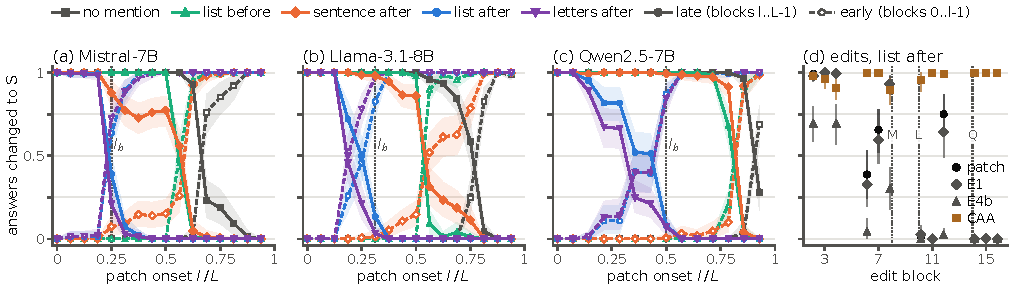
\includegraphics[width=\textwidth]{figures/fig_window.pdf}
  \caption{\textbf{With the candidates listed after the story, a patch of the writing token's cache must reach its early layers to change the answer.} Stage 9. (a--c)~Share of generated answers changed to S's value by the late patch (from block $l$ up; solid) and the early patch (below $l$; dashed), against $l/L$, by format (\NqStories{} new stories; 95\,\% two-stage cluster intervals as bands); dotted: $l_b$. (d)~Share of \fmtListA{} answers changed by edits at blocks 3--15: the natural patch, single-site steering (E1), the trained remap (E4b; not run at Llama) and steering at every position (CAA); per block, Mistral-7B, Llama-3.1-8B and Qwen2.5-7B from left to right; dotted: $l_b$ (M, L, Q: blocks \NqLbMistralSeven, \NqLbLlamaEight, \NqLbQwenSeven; \NqCores{} edit cores).}
  \label{fig:window}
\end{figure*}

\section{A match at the later mention, read by key}\label{sec:claim2}

\textbf{In two 7B models (Qwen2.5-7B, Mistral-7B), the reader heads match the writing token's key at the later mention of the written value and write a flag into that mention's row, which the answer reads by key.} The flag can move the answer but is neither specific nor the only carrier, and the question sets the sign of the read (\cref{app:claim2-brief}).

\paragraph{Two hops.}
In the discovery sample, the 5\,\% of heads whose attention from the option words to the writing token most follows its clamped key (hop~1), the \emph{reader heads}, recover \HoneRQwenSeven{} and \HoneRMistralSeven{} of the option rows' read when only they see it (\cref{app:heads}). They are enriched for duplicate-token heads \citep{wang2022ioi} (exploratory). Mean-ablating them at the option rows leaves \HthreeRhoQwenSeven{} and \HthreeRhoMistralSeven{} of the key read and raises the value read: a copy route stays available. The answer reads the option words (hop~2), mainly by key, not the writing token: in lists the written value is read at its later mention.

\paragraph{What the readers write.}
The reader heads write one vector per layer into the re-mentioned word's row. We call it the \emph{flag}. Injected with no key clamp into the row of an option absent from the story, a version fit without that word moves the answer there, with \ci{\JdOneRatioQwenSeven}{\JdOneRatioQwenSevenLo}{\JdOneRatioQwenSevenHi} and \ci{\JdOneRatioMistralSeven}{\JdOneRatioMistralSevenLo}{\JdOneRatioMistralSevenHi} of the key read's identity effect (Qwen2.5-7B, Mistral-7B; the answer changes in \pct{\JdOnePiXQwenSeven} and \pct{\JdOnePiXMistralSeven} of stories); like the natural key clamp, the injection adds the flag at that row and removes it at the base value's row. Its mean direction names no candidate. The answer reads it by key, as it reads the natural one (giving only the answer row the option rows' original keys removes \JdFourKQwenSeven{} and \JdFourKMistralSeven{} of its effect). It is not specific: structured controls also move the answer (at Qwen2.5-7B the mean reader output, which overlaps the flag, \JdTwoRatioMeanHQwenSeven{} as much as the flag; at Mistral-7B the heads' own write with the flag removed, \JdTwoRatioOrthMistralSeven). Nor is it the only carrier: removing it, one direction per layer, leaves \ci{\JdThreeRhoFlagQwenSeven}{\JdThreeRhoFlagQwenSevenLo}{\JdThreeRhoFlagQwenSevenHi} and \ci{\JdThreeRhoFlagMistralSeven}{\JdThreeRhoFlagMistralSevenLo}{\JdThreeRhoFlagMistralSevenHi} of the key read, and at Qwen two control directions that overlap it also remove part of the read (they leave \JdThreeRhoPconeQwenSeven{} and \JdThreeRhoMeanHQwenSeven; \cref{app:flag}).

\paragraph{The sign of the read.}
Asked which option was \emph{not} mentioned, both reads turn negative and the same reader heads carry them; that the sign is applied after the first hop is exploratory. In indirect-object identification (IOI) with the names re-mentioned in a parenthesis, the key read is negative and the value read positive in both models, consistent with S-inhibition \citep{wang2022ioi}, and the negative read is applied where the answer reads the listed names, more by key than by value (restoring their keys and values for the answer row alone removes \JdRouteKVQwenSeven{} and \JdRouteKVMistralSeven{} of it). The ten answer-side heads ranked in lists carry almost none of it: a different (or a distributed) reader applies the negative read. The belief readers carry the IOI read at Qwen2.5-7B; at Mistral-7B a gate failed. The flag is written in sentences as in lists at 1.5B--7B; whether it carries the size of the sentence read across scale is unresolved (on the preregistered ratio the injected and natural reads differ, on a post hoc contrast they agree; \cref{app:scale}), and at 1.5B it is read by key rather than by value. At Qwen2.5-7B the initial-state flag does not carry binding separably from sentence order (at Mistral-7B it does, fragilely), and a key naming no candidate removes more support for the base value than removing its flag (\cref{app:sign,app:flag}).
